\chapter{Use Case 1: WorldData Explorer}

\section{Einführung}
Im ersten Use Case geht es hauptsächlich um die Anzeige grosser Datenmengen auf der Karte. Dazu importieren wir bestehende Datenbestände in die Google Fusion Tables und visualisieren diese mittels Google Maps API auf der Karte.

\subsection{Ziel}
Es sollen verschiedene historische Länderdaten auf einer Weltkarte angezeigt werden. Die Daten sind pro Jahr und Thema unterteilt. Über eine Zeitachse soll es möglich sein die Daten der verschiedenen Jahre zu selektieren. Eine solche Darstellung kann beispielsweise dabei helfen Zusammenhänge zwischen verschiedenen Themenbereichen zu finden.

\subsection{Vorgehen}
Um die Daten pro Land zu visualisieren, werden zuerst die Landesgrenzen als Geometrie-Datensätze in eine separate Fusion Tabelle importiert. In eine andere Tabelle werden dann die Daten importiert unterteilt nach Land und Jahr. Diese beiden Tabellen werden per Merge-Funktion zu einer Tabelle zusammengefasst, welche dann mittels FusionTablesLayer auf der Karte dargestellt werden kann.

\subsubsection{ERD}
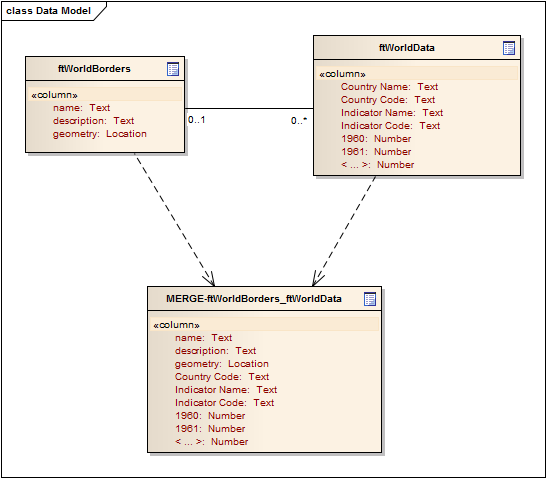
\includegraphics[scale=0.8]{images/usecase1-worlddata-erd.png}

\subsection{Datenquellen}
Als Datenquelle wurde der Daten Katalog der Weltbank (\url{http://data.worldbank.org/}) verwendet. Darin finden sich länderspezifische Daten aufgeteilt in über 7000 Themenbereiche.

Die Landesgrenzen wurden als \gls{KML}-Datei von einer inoffiziellen Google Earth Library-Webseite (\url{http://www.gelib.com/world-borders.htm}) bezogen. 

\section{Anforderungsspezifikation}

\section{Analyse}

\section{Design}

\section{Implementation}

\section{Test}

\section{Resultate}

\section{Weiterentwicklung}

\section{Benutzerdokumentation}
\subsection{Importieren der Daten in Google Fusion Tables}
\subsubsection{Landesgrenzen}
Die Landesgrenzen liegen als KML-Datei vor. Diese beinhaltet alle Länder mit ihren Grenzen definiert als Polygone.

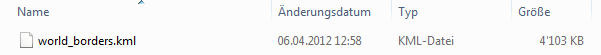
\includegraphics{images/usecase1-worlddata/worlddata-worldborders_kml.png}

\begin{enumerate}
\item Google Docs öffnen (\url{https://docs.google.com/}) und sich mit seinem Google Account einloggen
\item Erstellen > Tabelle (Beta) \\ 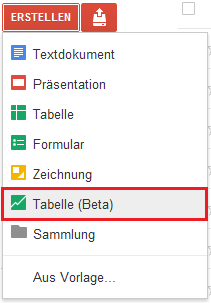
\includegraphics{images/usecase1-worlddata/worlddata-worldborders_import1.png}
\item Es öffnet sich die neue Fusion Table mit dem Dialog zum Importieren von bestehenden Daten
\item Im Tab \emph{From this computer} die lokal gespeicherte Datei auswählen > Next
\item Die Daten werden automatisch in passende Spalten eingeteilt
\item Abschliessend muss der Tabelle noch einen Namen gegeben werden
\item Mit \emph{Finish} werden die Daten dann importiert
\end{enumerate}

Die Tabelle sollte nun folgendermassen aussehen:

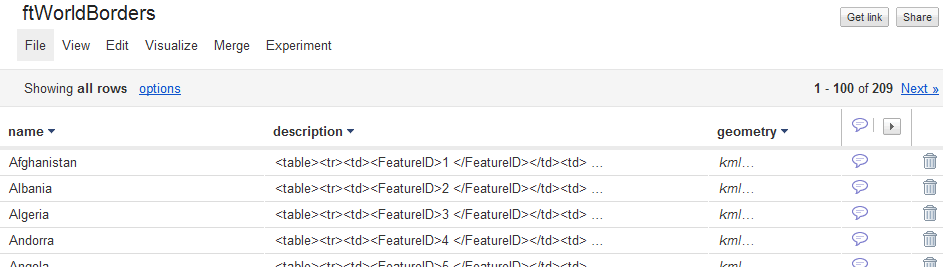
\includegraphics[scale=0.65]{images/usecase1-worlddata/worlddata-worldborders_import_done.png}

\subsubsection{Daten}
Die Daten liegen als CSV-Datei vor. Diese beinhaltet folgende Spalten:
\begin{itemize}
\item Country Name
\item Country Code
\item Indicator Name
\item Indicator Code
\item 1960
\item 1961
\item ...
\end{itemize}

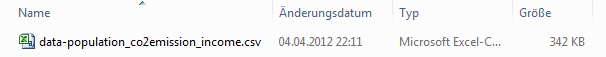
\includegraphics{images/usecase1-worlddata/worlddata-data_csv.png}

Das Vorgehen für den Import der Daten ist dasselbe wie bei den Landesgrenzen.

Die Tabelle sollte nun folgendermassen aussehen:

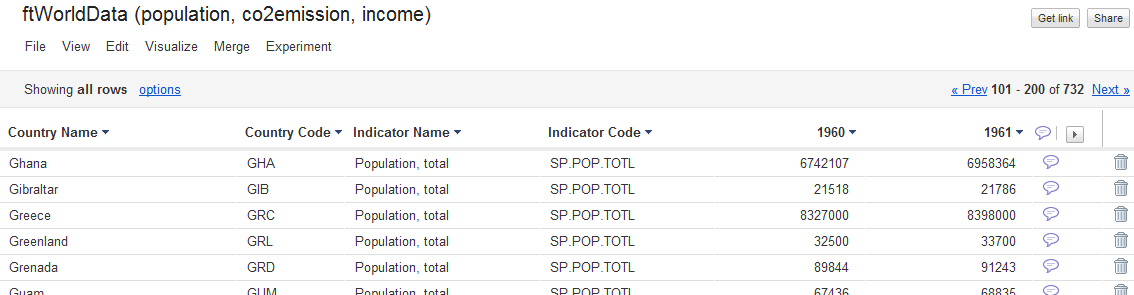
\includegraphics[scale=0.5]{images/usecase1-worlddata/worlddata-data_import_done.png}

\subsubsection{Tabellen mergen}
Sind beide Fusion Tables erstellt müssen diese zusammengefügt werden, um sie schlussendlich als einen einzelnen Layer auf der Karte darzustellen. Dazu bietet Google Fusion Tables die \emph{Merge}-Funktion an. 

\begin{enumerate}
\item Eine der beiden Tabellen öffnen
\item Im Menü \emph{Merge} auswählen \\ 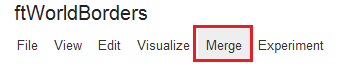
\includegraphics{images/usecase1-worlddata/worlddata-merge1.png}
\item Es öffnet sich ein Popup, welches durch den Vorgang führt
\item In der 1. Spalte wählt man die Spalte aus, über welche die beiden Tabellen verbunden werden sollen. In unserem Fall ist dies die Spalte mit den Namen der Länder.
\item In der 2. Spalte muss man zuerst die andere Tabelle auswählen und dann ebenfalls die Spalte, in welcher die Namen der Länder gespeichert sind.
\item Schlussendlich muss der neuen Tabelle ein Namen gegeben werden
\item Mit einem Klick auf \emph{Merge tables} wird die neue Tabelle mit den zusammengefügten Daten erstellt. \\ 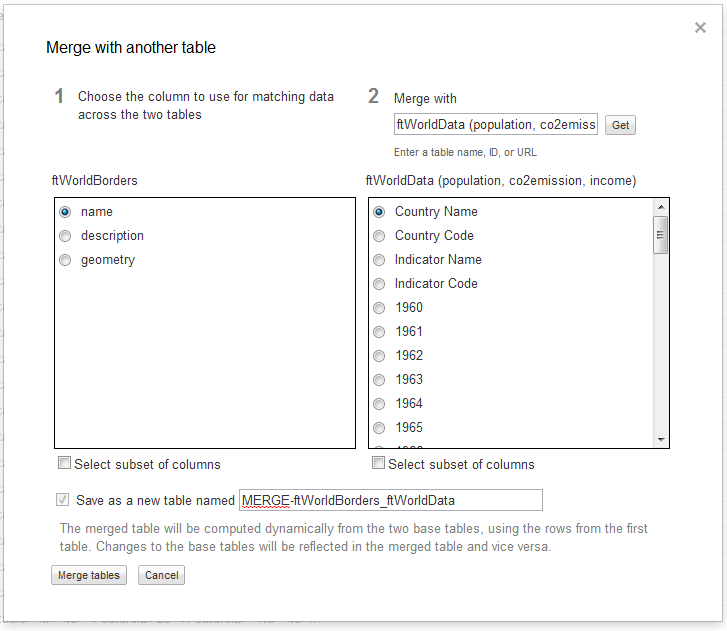
\includegraphics[scale=0.8]{images/usecase1-worlddata/worlddata-merge2.png}
\end{enumerate}

Die zusammengeführte Tabelle sollte nun folgendermassen aussehen:

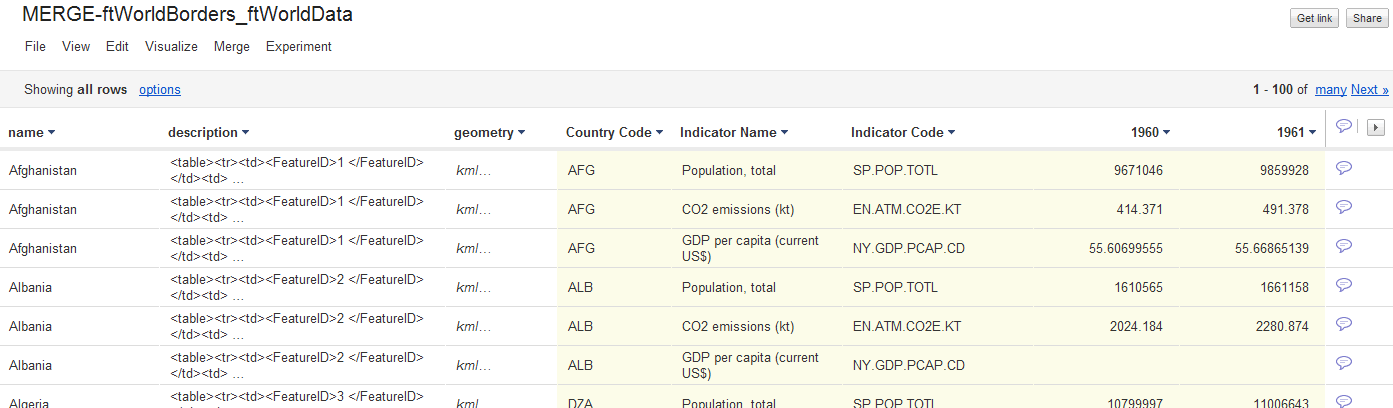
\includegraphics[scale=0.4]{images/usecase1-worlddata/worlddata-merge_done.png}

\subsubsection{Merge-Tabelle für die Verwendung mit FusionTablesLayer vorbereiten}
Um die Tabelle nun als FusionTablesLayer verwenden zu können, muss diese als \emph{öffentlich} markiert werden. Dazu klickt man bei der geöffneten Tabelle auf den \emph{Share}-Button in der linken oberen Ecke.

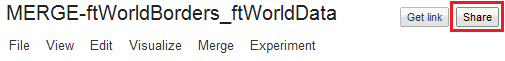
\includegraphics{images/usecase1-worlddata/worlddata-prepare_fusiontableslayer1.png}

Im Dialogfenster wählt man unter \emph{Visibility options} den Eintrag \emph{Public} aus.

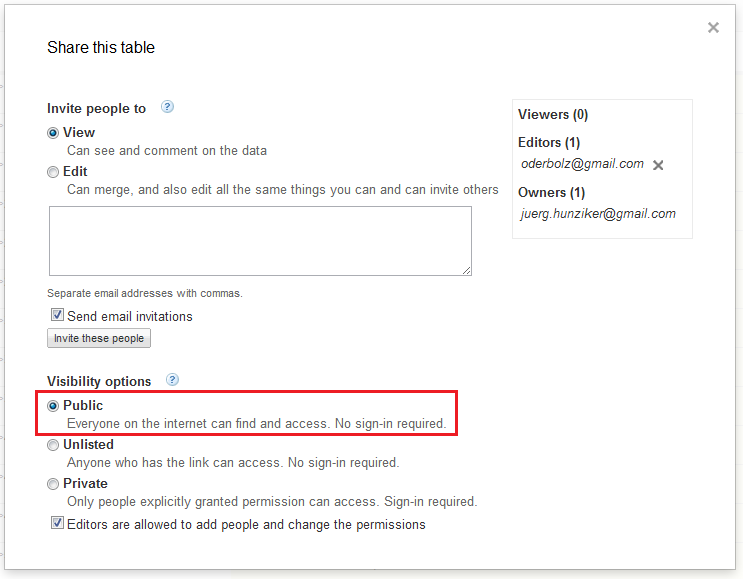
\includegraphics[scale=0.8]{images/usecase1-worlddata/worlddata-prepare_fusiontableslayer2.png}

Als letzten Schritt muss man sich noch die eindeutige ID der Tabelle merken. Dazu wählt man im Menü  \emph{File > About} und kopiert sich die angezeigte \emph{Numeric ID} im geöffneten Dialog.

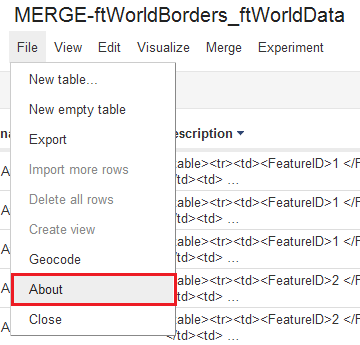
\includegraphics{images/usecase1-worlddata/worlddata-prepare_fusiontableslayer3.png}

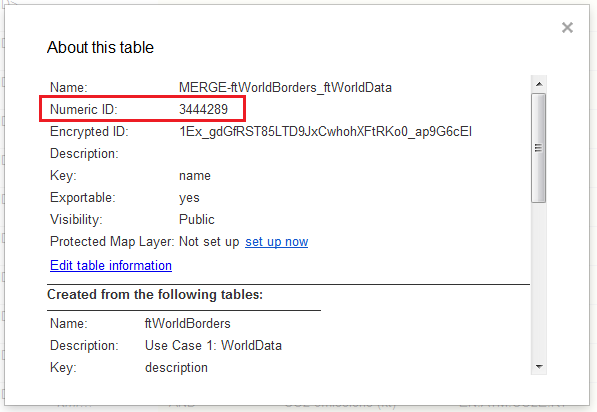
\includegraphics{images/usecase1-worlddata/worlddata-prepare_fusiontableslayer4.png}

\subsection{Konfiguration der Applikation}
